\begin{figure}[htbp]
	\centering

    \subfloat[Parameter space plot, \acs{SCT}, $\sigma_n=1068$ Pa, P=0.8.]{
	  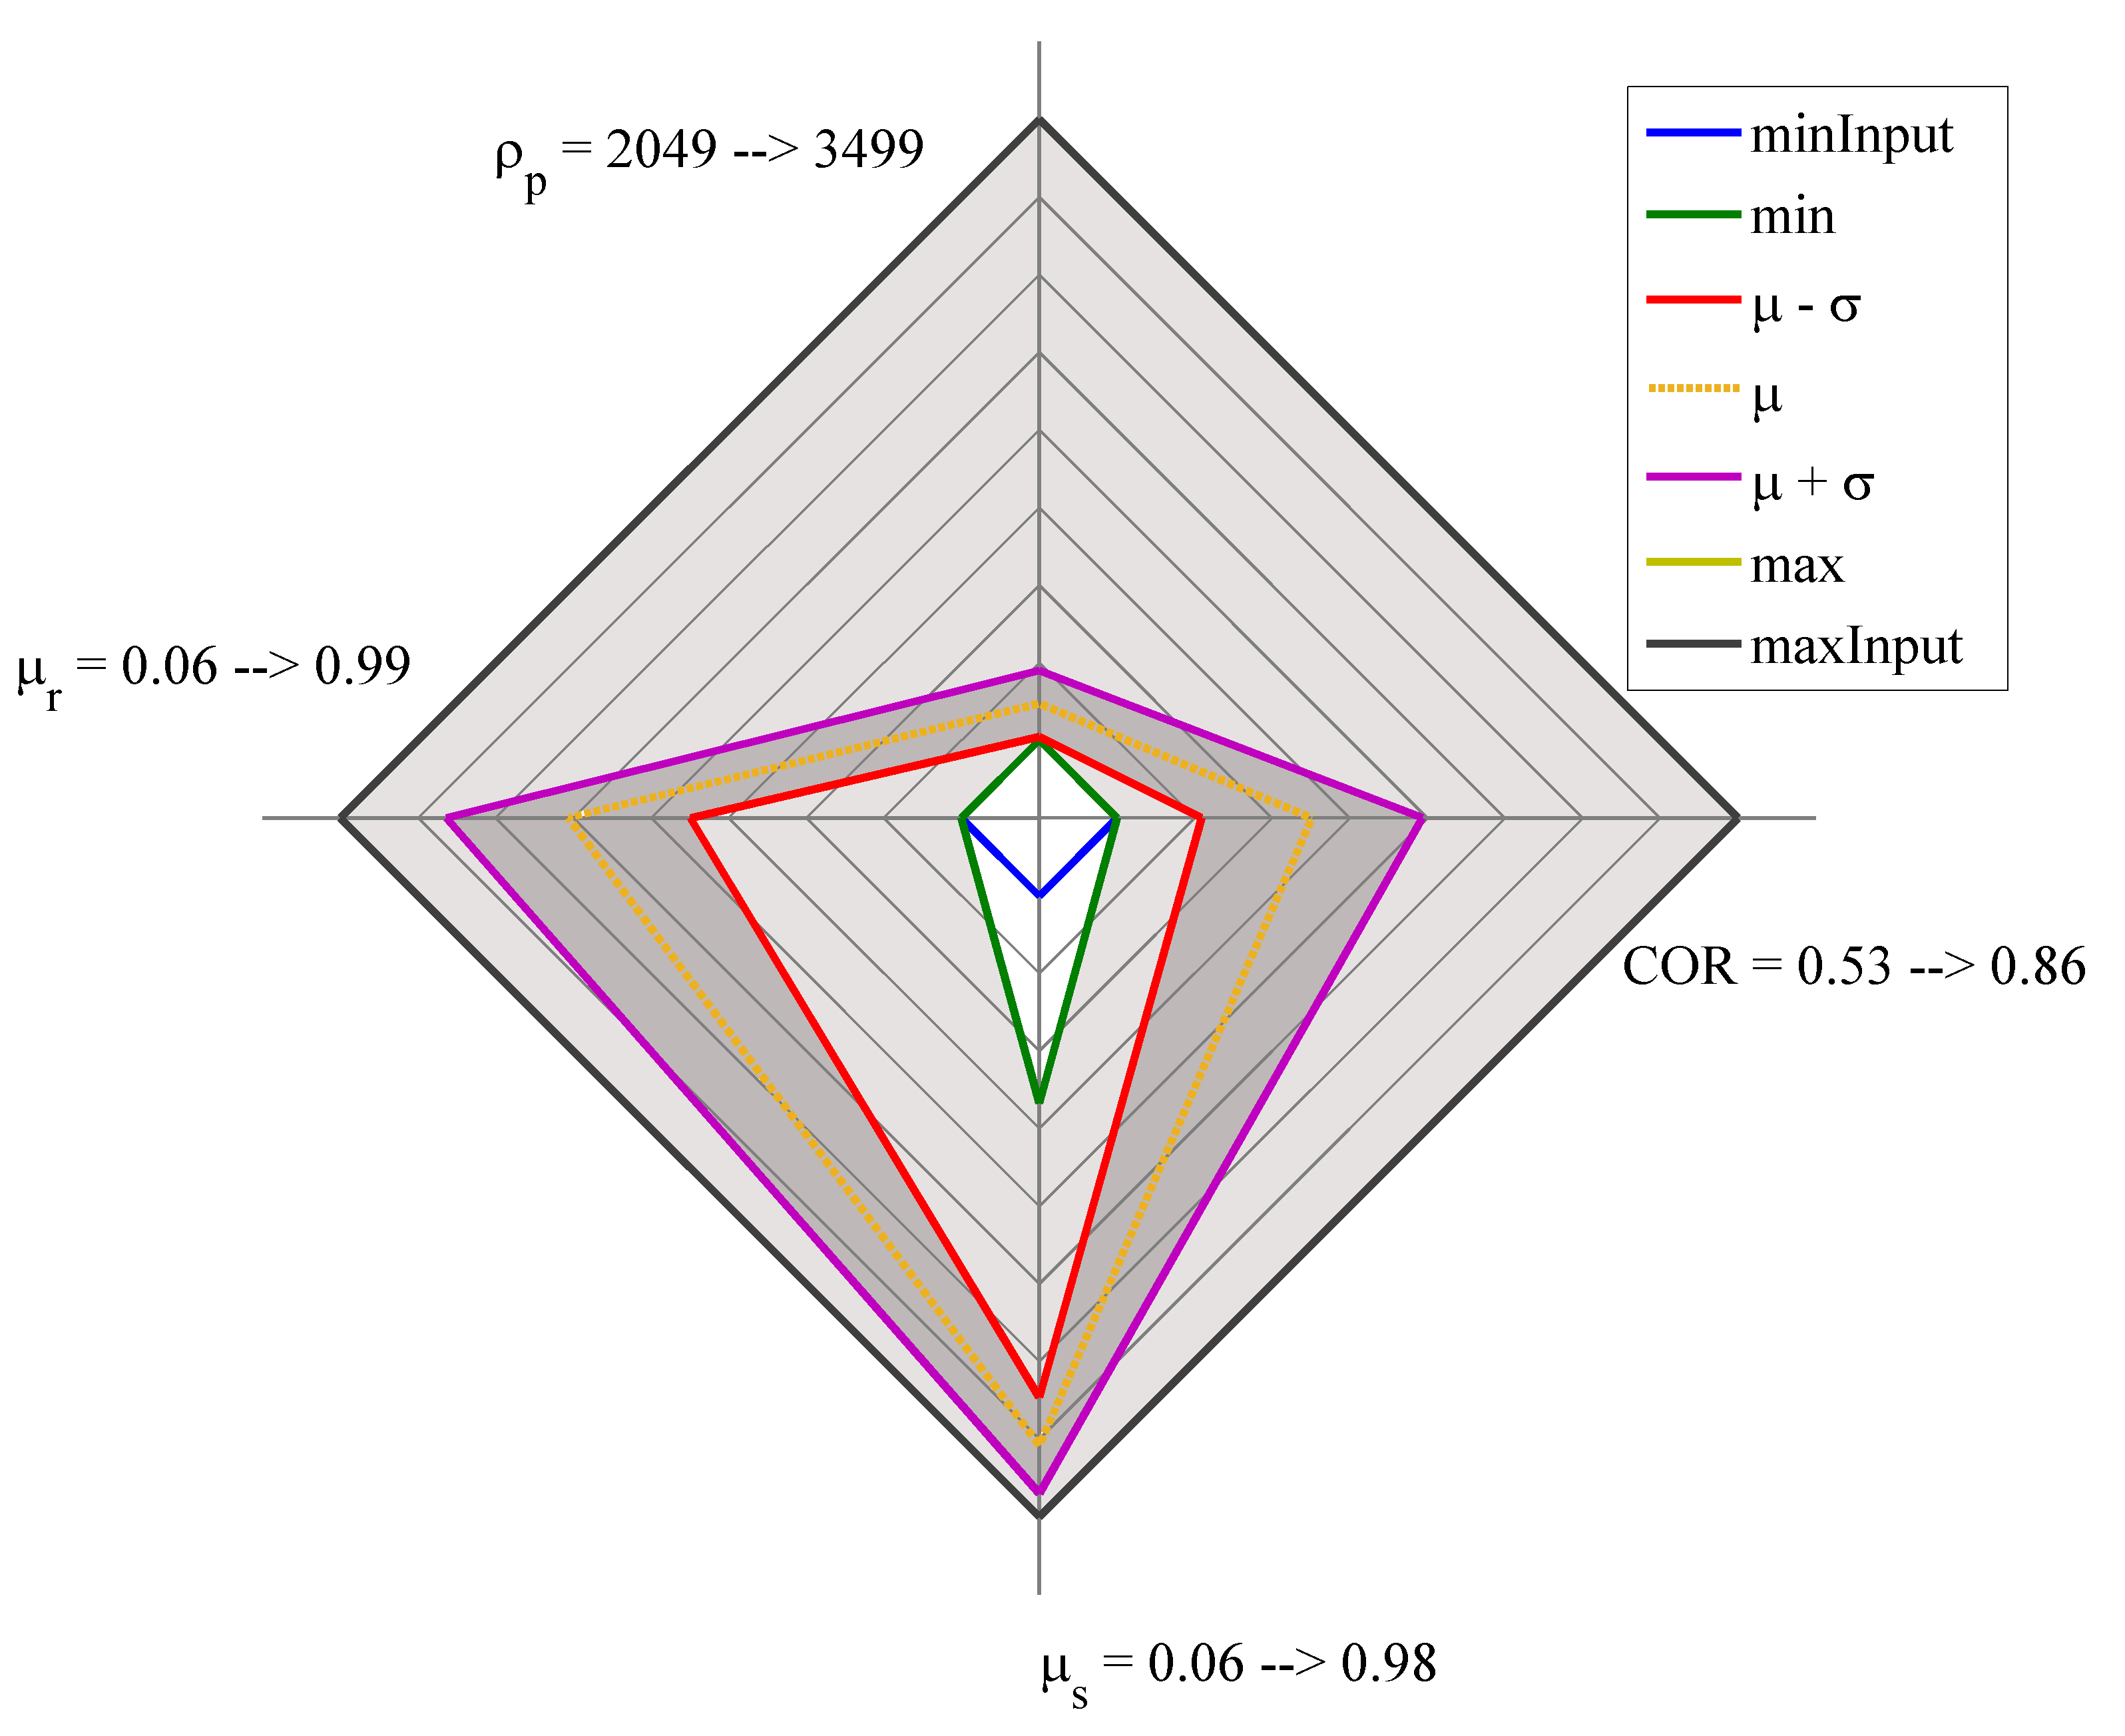
\includegraphics[width=.5\columnwidth]{images/150ParamSpaceSCT1068p08sinterfine}
	  \label{fig:150ParamSpaceSCT1068p08sinterfine}  }
	 
    \subfloat[Parameter space plot, \acs{SCT}, $\sigma_n=1068$ Pa, P=1.0.]{
	  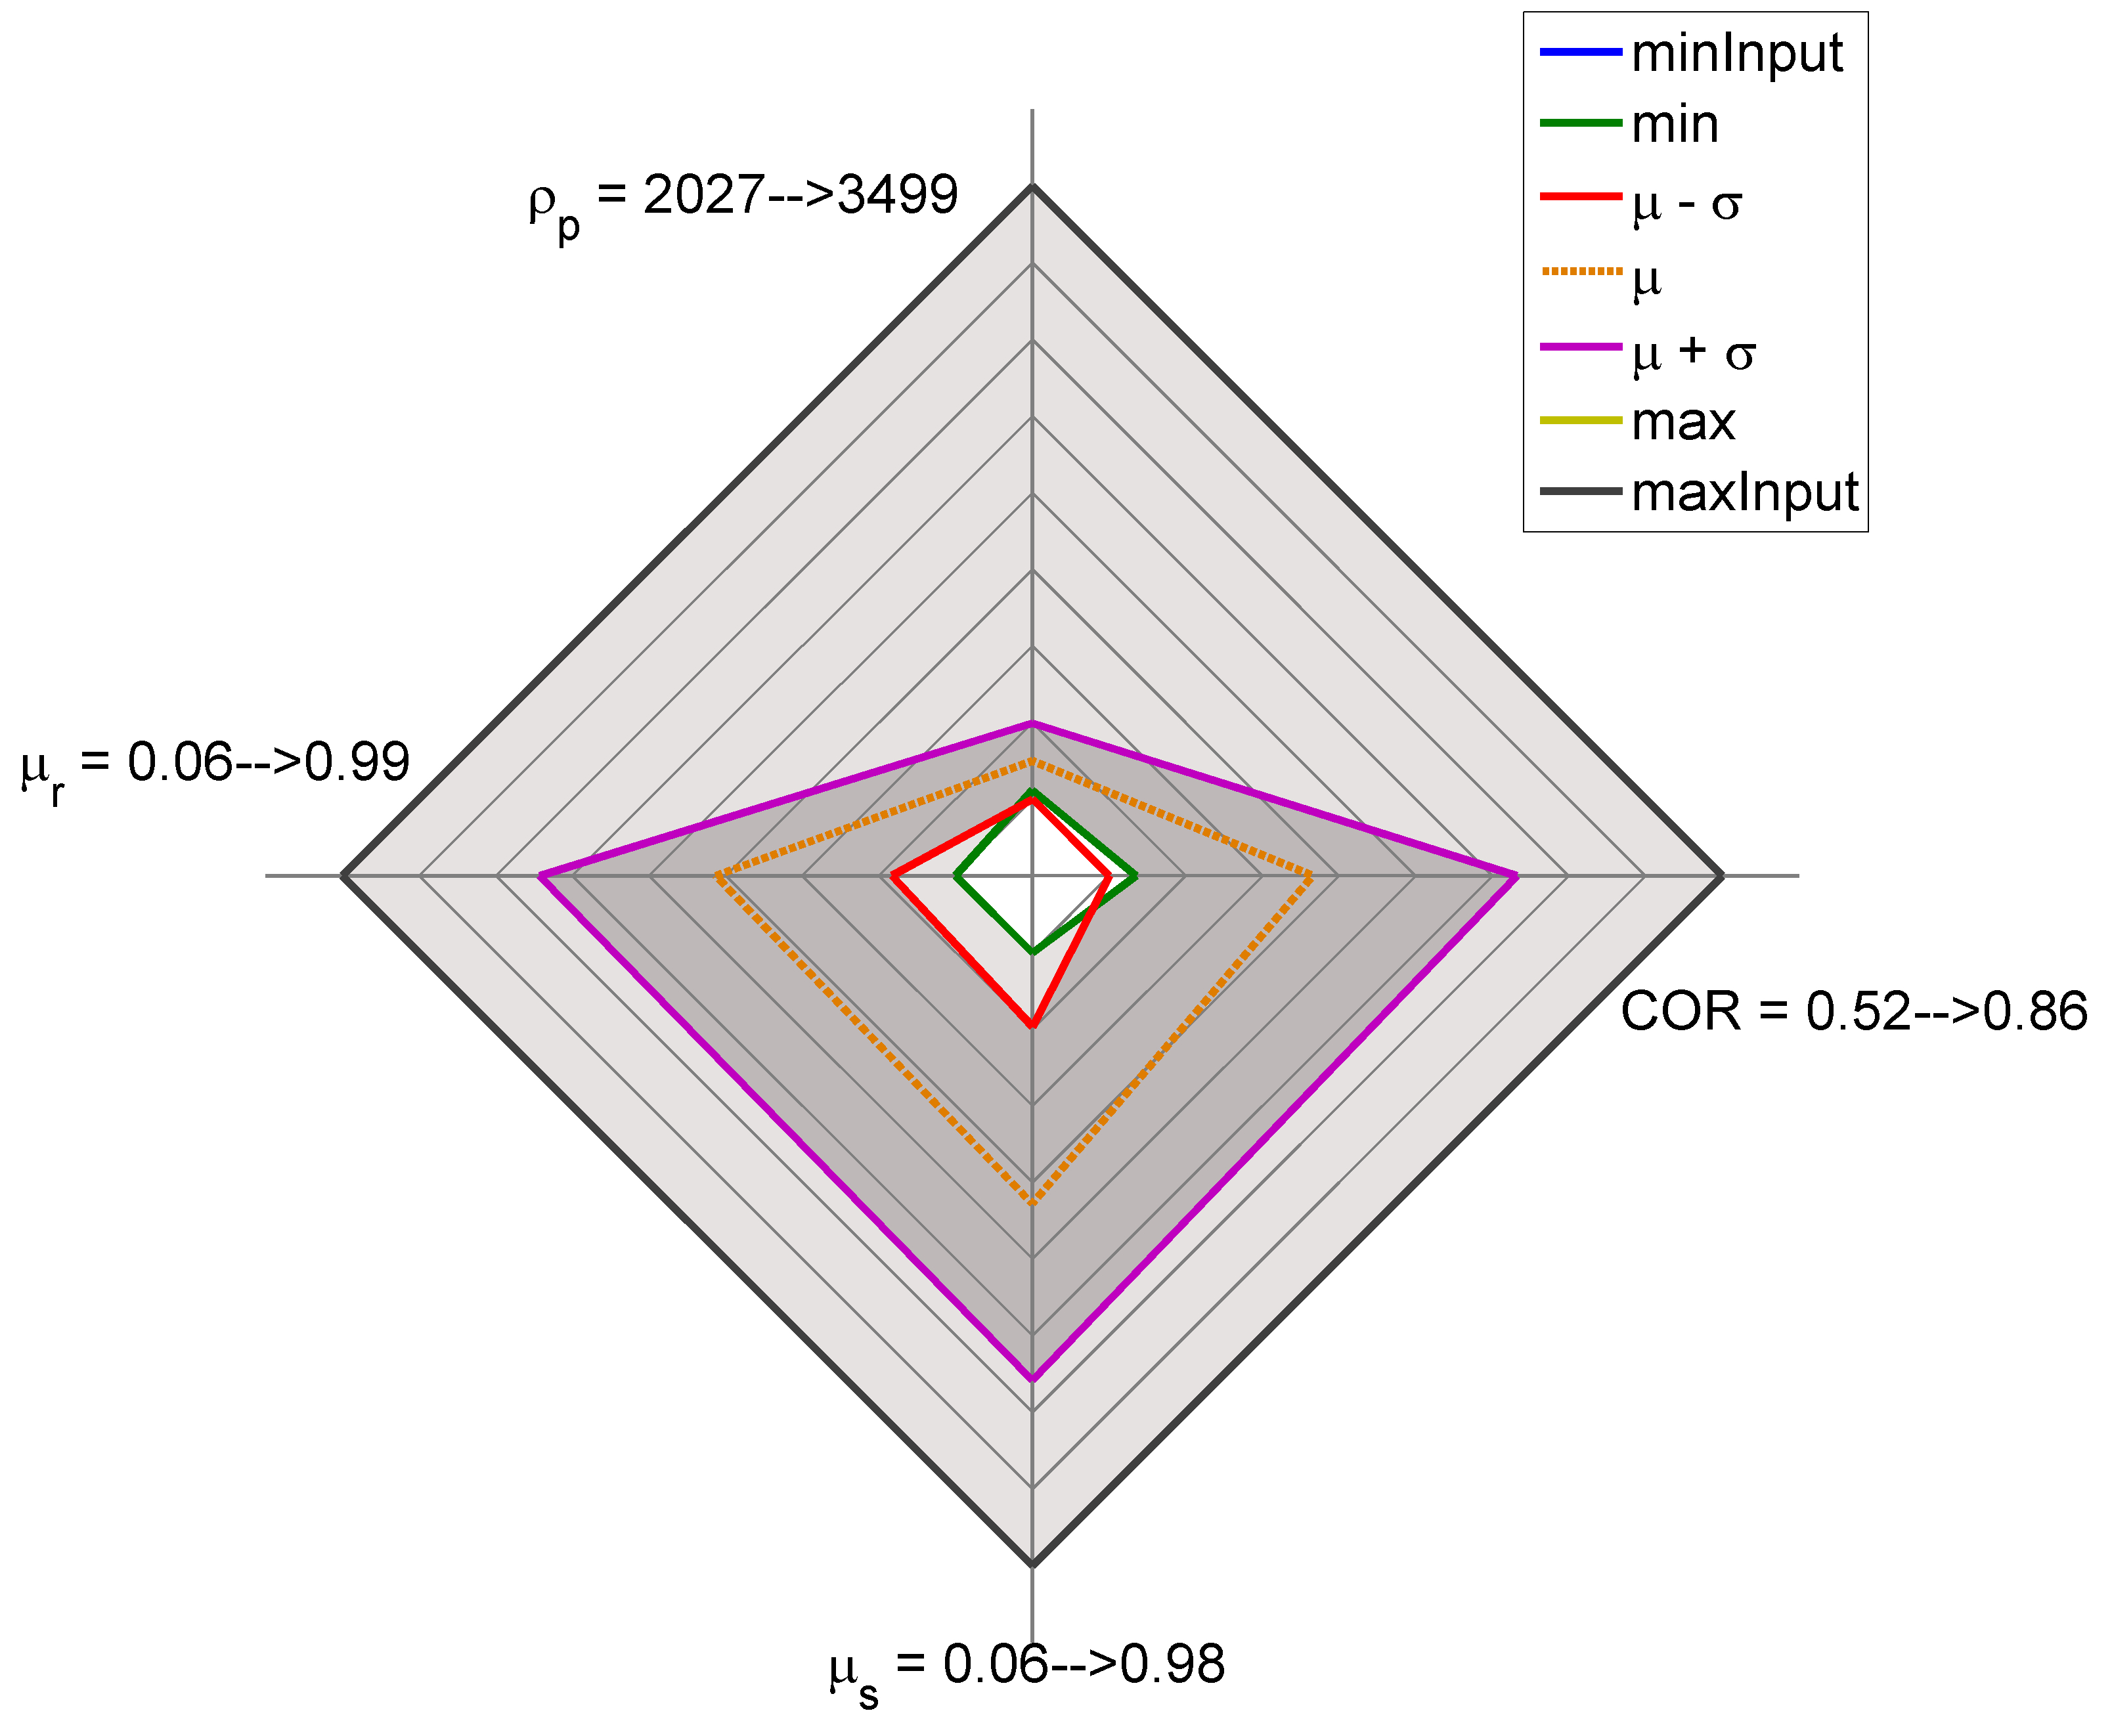
\includegraphics[width=.5\columnwidth]{images/041radarpirker1schulze1068}
	  \label{fig:041radarpirker1schulze1068}  } 
	  
    \subfloat[Parameter space plot, \acs{SCT}, $\sigma_n=1068$ Pa, P=1.2.]{
	  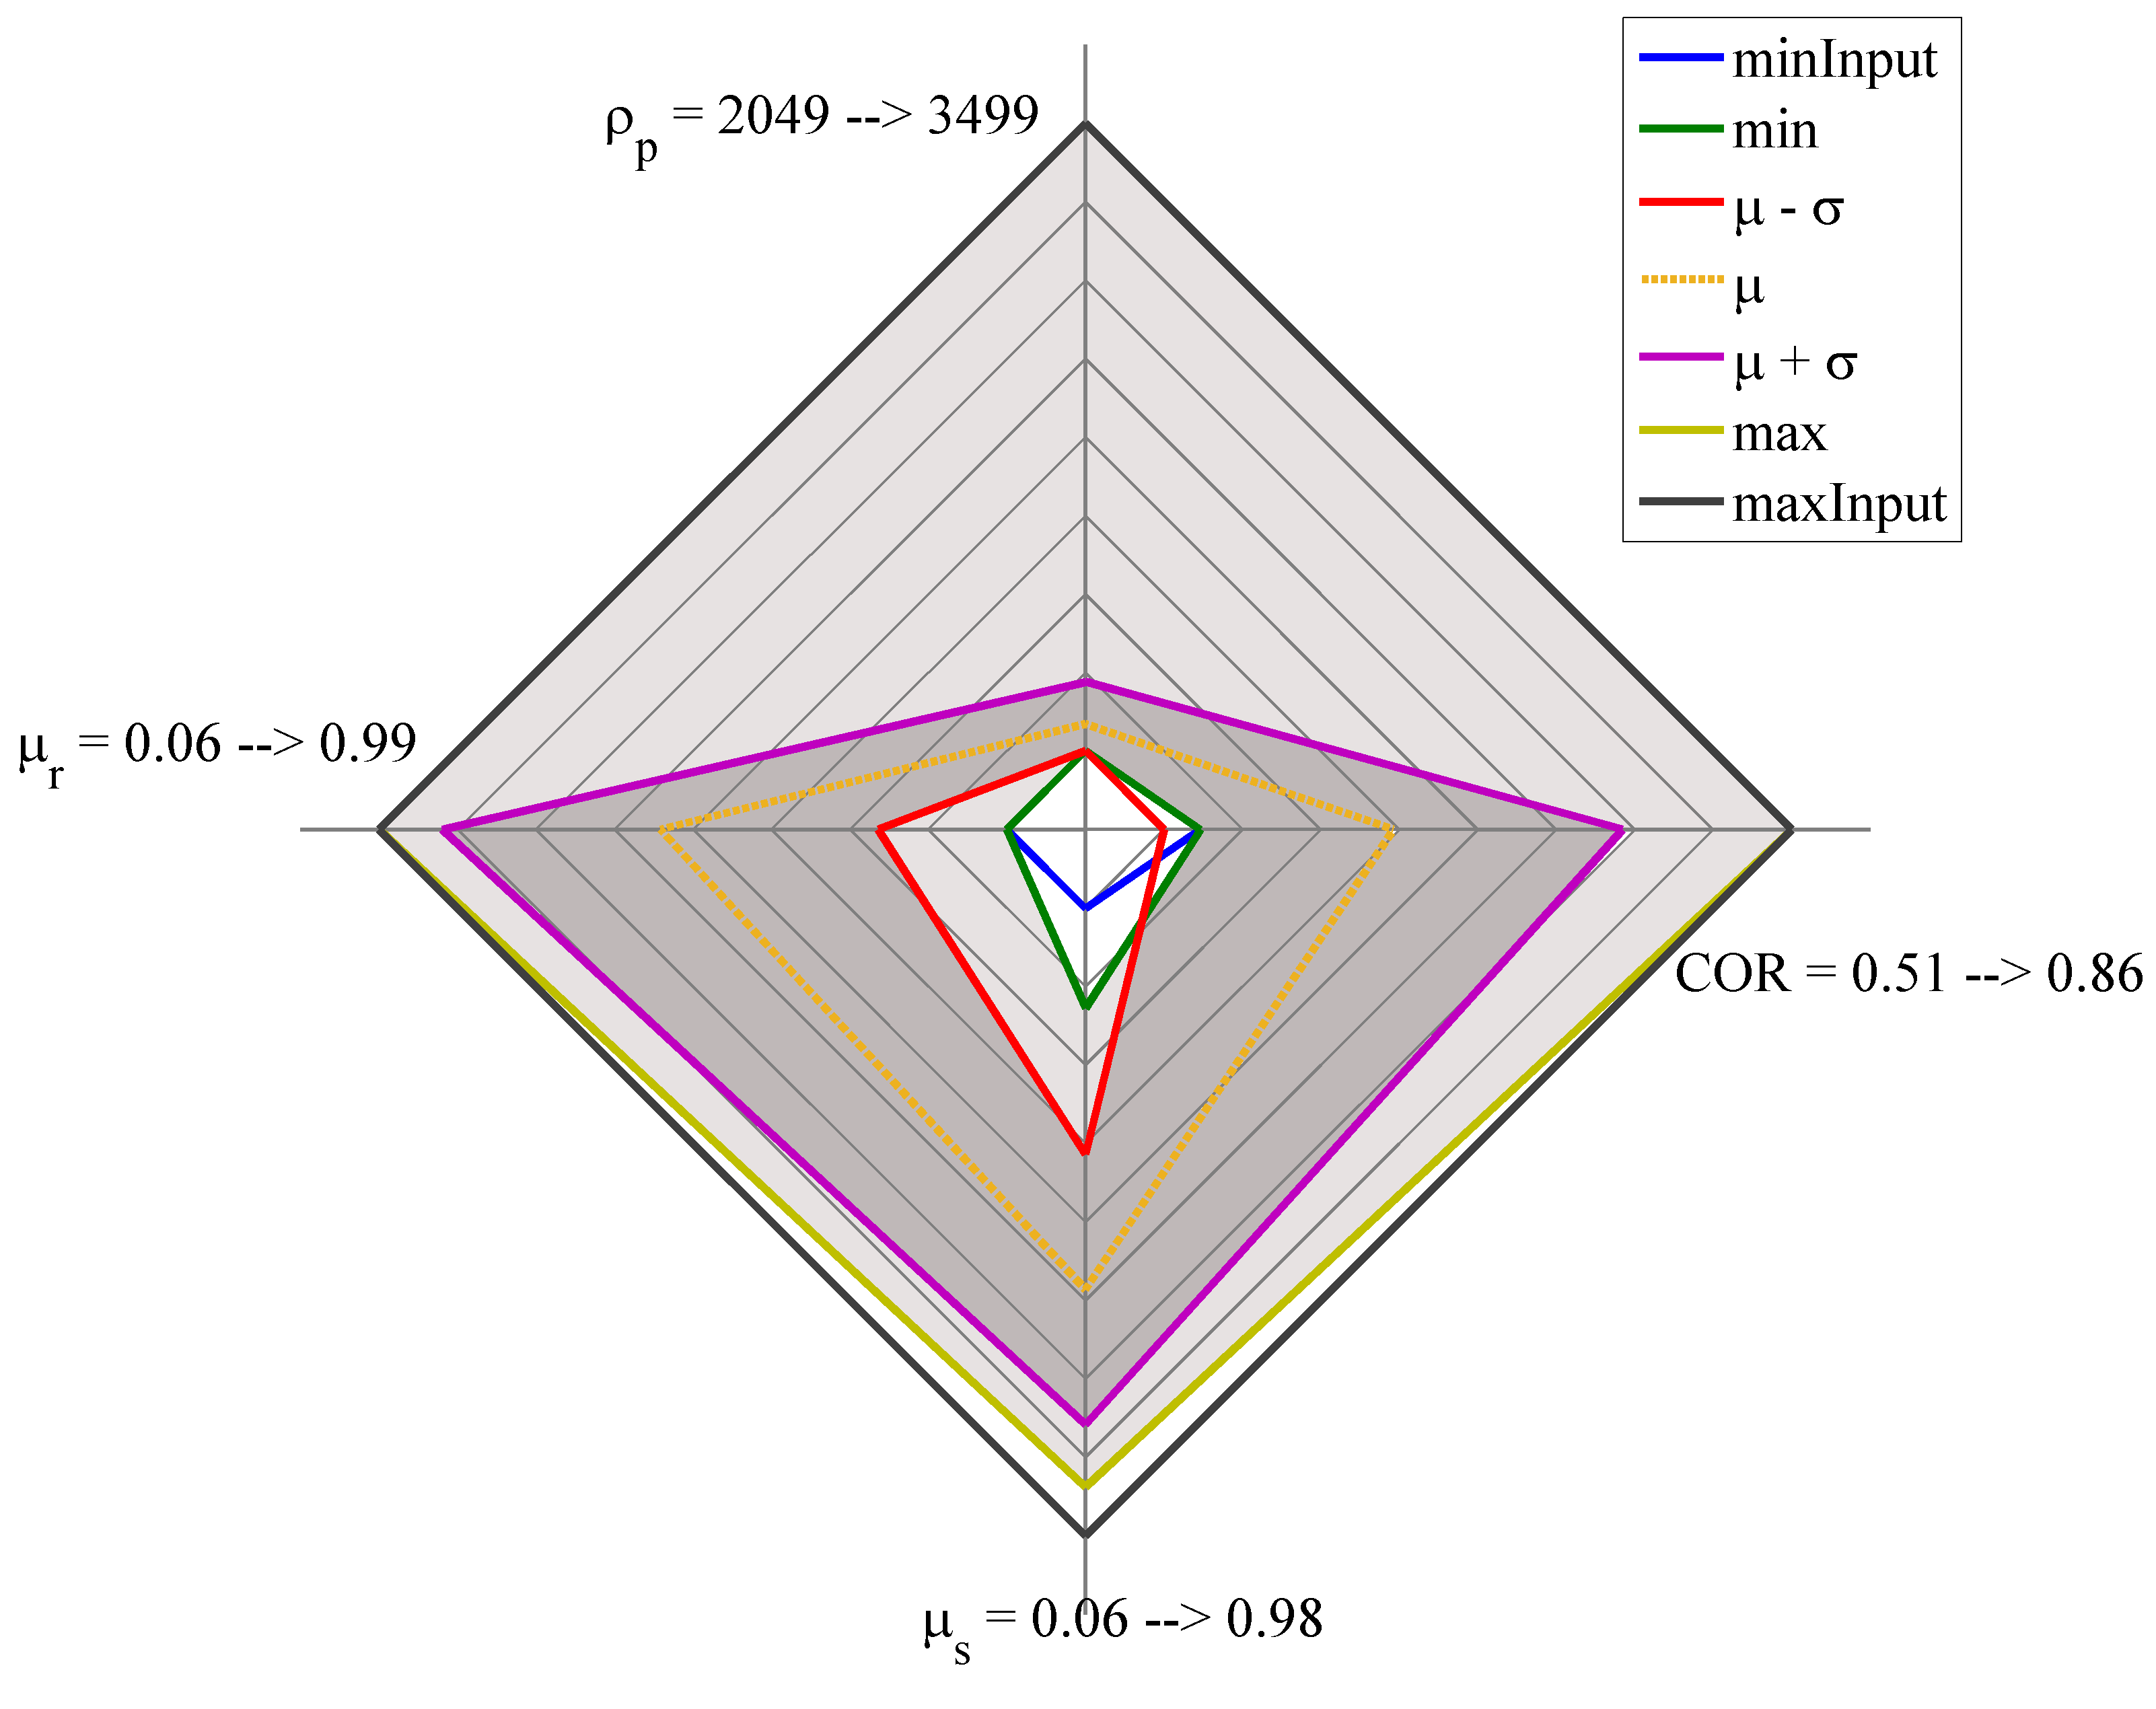
\includegraphics[width=.5\columnwidth]{images/151ParamSpaceSCT1068p12sinterfine}
	  \label{fig:151ParamSpaceSCT1068p12sinterfine}  } 	  
	  

 % \hfill\null
  \caption[SCT parameter space plots 1]{SCT parameter space
  plots for sinter fine, $\sigma_n=1068$ Pa.}
  \label{fig:149paramspaceplotsct1068}
\end{figure}

% \begin{figure}%[!h] 
% \centering 
% 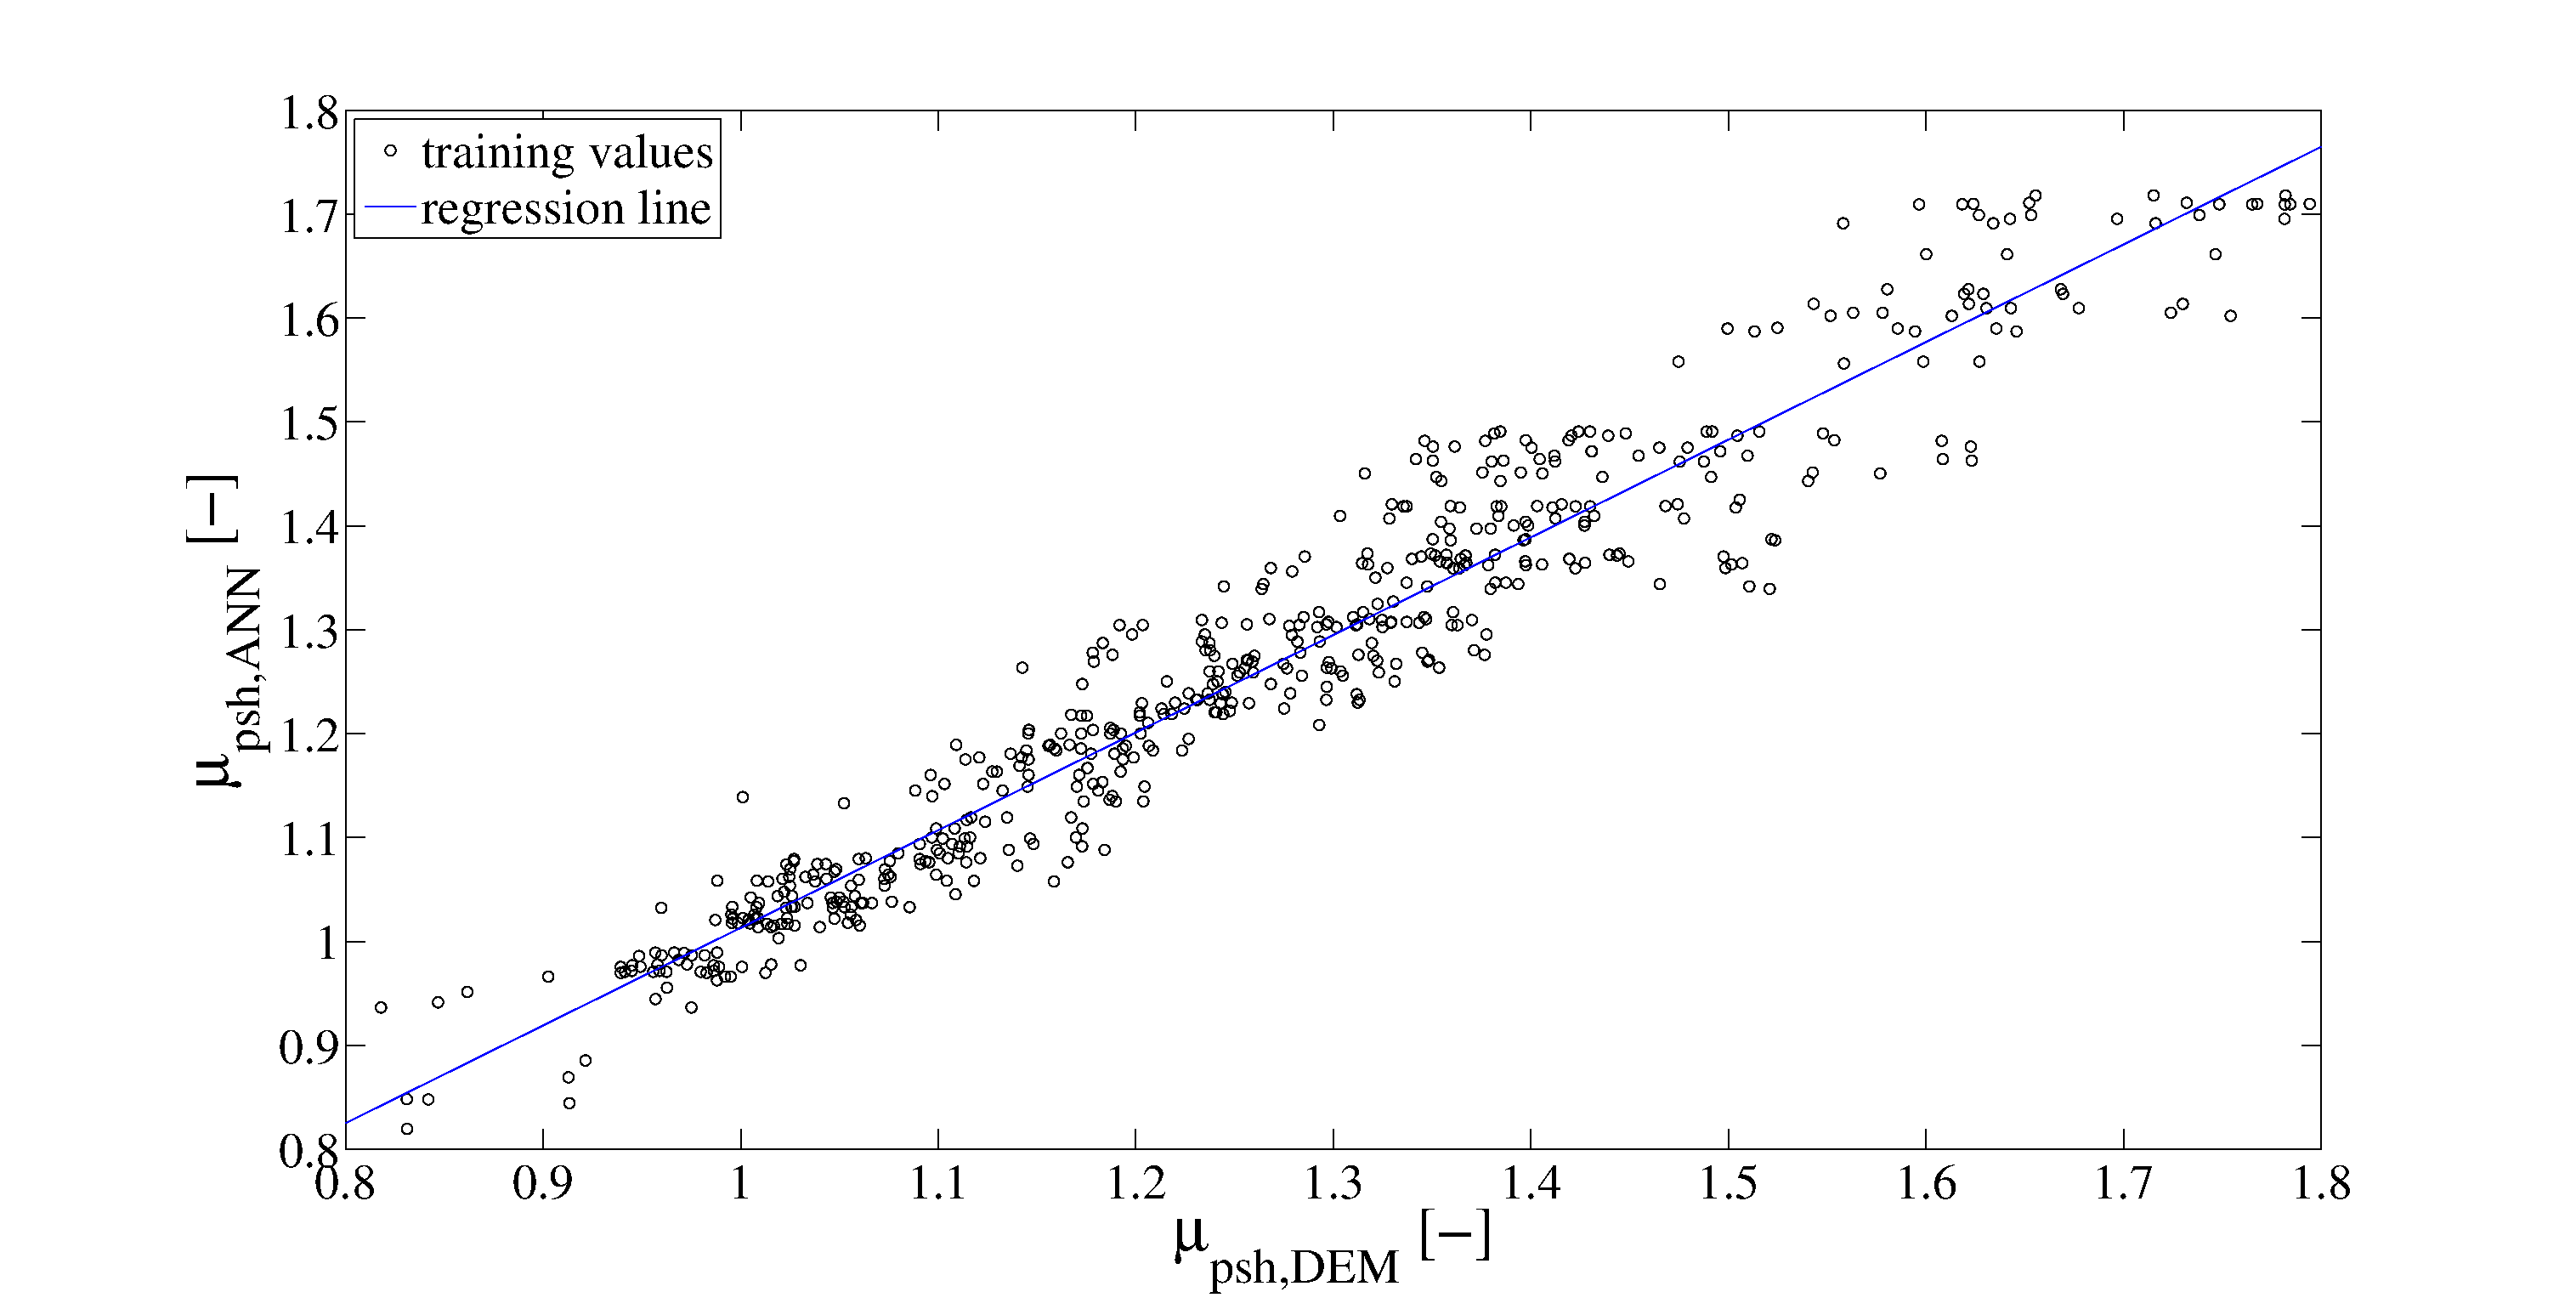
\includegraphics[width=.80\columnwidth]{images/022regression.eps}
% %[width=.48\textwidth]
% \caption[Comparison between prediction of the trained ANN and full DEM
% simulation]{Comparison between prediction of the trained Artificial Neural
% Network (\acs{ANN}) and 546 
% \wrong{write down all the simulations performed at the end.}
% full DEM simulations of the coefficient of pre-shear
% (\acs{mupsh}).}
% \label{fig:022regression} 
% \end{figure}